

The following games are a mix of game theory applied to communication networks and security games, as well as others that did not fit elsewhere.


\begin{example}\label{ex.chasnov20.5.2}
A general-sum 2-player game in $1 \times 1$ variables constrained to the torus
\begin{equation*}
x_{i1} \in [-\pi, \pi] \quad \forall i \in \{1, 2\}
\end{equation*}
with utilities parameterized by $\phi = \left(0, \frac{\pi}{8}\right), \alpha = (1, 1.5)$:
\begin{align*}
u_1(x_1, x_2) &= \alpha_1 \cos(x_{11} − \phi_1) - \cos(x_{11} - x_{21})\\
    u_2(x_1, x_2) &= \alpha_2 \cos(x_{21} − \phi_2) - \cos(x_{21} - x_{11})
\end{align*}
This game appeared in a paper by \textcite[5.2]{chasnov.ratliff.ea:convergence}, who reported  pure equilibria at $(-1.063, 1.014)$ and $(1.408, -0.325)$.
\end{example}

\noindent
\begin{minipage}[c]{0.55\textwidth}
\begin{example}\label{ex.chasnov20.b.1}
A two-player zero-sum game in $1 \times 1$ variables constrained to the interval
$$x_{i1} \in [0,1] \quad \forall i \in \{1, 2\}.$$
The utility function is
\begin{align*}
u_{1}\left( x_{1}, x_{2} \right) &= \sigma(x_2)^\top A \sigma(x_1)
\end{align*}
where $\sigma(x)$ is the \emph{softmax} vector
$$\sigma(x) = \left[\frac{e^{10x}}{e^{10x}+e^{10(1-x)}},\frac{e^{10(1-x)}}{e^{10x}+e^{10(1-x)}}\right]$$
This is a continuous version of the classical matching-pennies game, and it was studied by \textcite[B.1]{chasnov.ratliff.ea:convergence}, who reported a pure equilibrium at $(x_{11}, x_{21}) = (0.5, 0.5)$.
\end{example}
\strut
\end{minipage}
\hfill
\begin{minipage}[c]{0.35\textwidth}
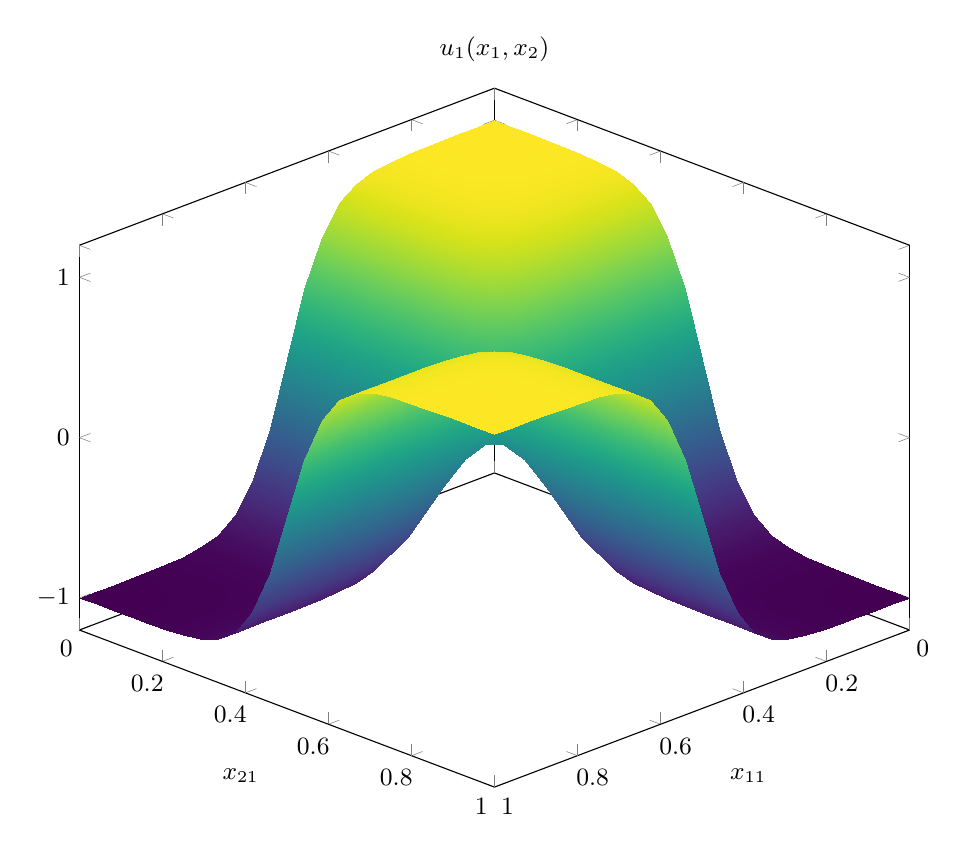
\begin{tikzpicture}
\begin{axis}[
    font=\small,
    domain=0:1,
    y domain=0:1,
    xlabel=$x_{11}$,
    ylabel=$x_{21}$,
    title={$u_1(x_1,x_2)$},
    colormap/viridis,
    view={135}{30},
    mesh/ordering=y varies,
    width=\textwidth,
]
\addplot3[
    surf,
    shader=interp,
]
{
    (
        (exp(10*y) / (exp(10*y) + exp(10*(1 - y))) - exp(10*(1 - y)) / (exp(10*y) + exp(10*(1 - y))))
        *
        (exp(10*x) / (exp(10*x) + exp(10*(1 - x))) - exp(10*(1 - x)) / (exp(10*x) + exp(10*(1 - x))))
    )
};
\end{axis}
\end{tikzpicture}
\end{minipage}


\begin{example}\label{ex.ratliff13.location}
A general-sum 2-player game in $1 \times 1$ variables on the interval
\[
x_i \in [-\pi, \pi] \quad \forall i \in \{1,2\}.
\]
The utility functions are given by
\begin{align*}
u_{1}\left( x_{1}, x_{2} \right) &= \cos\left( x_{11} \right) - \alpha_1 \cos\left( x_{11} - x_{21} \right) \\
u_{2}\left( x_{1}, x_{2} \right) &= \cos\left( x_{21} \right) - \alpha_2 \cos\left(  - x_{11} + x_{21} \right).
\end{align*}
\textcite[Location Game]{ratliff.burden.ea:characterization} studied this game with $\alpha = [1, 1.05]$, in which case the game has two NE: at $(x_1, x_2)$ equal to $(1,-1.1)$, or $(-1,1.1)$.
\end{example}

\begin{example}\label{ex.kroupa21.5}
A 3-player polynomial network game in $1 \times 1 \times 1$ variables on the interval
$$x_{i1} \in [0,1] \quad \forall i \in \{1,2,3\}.$$
The utilities \cite[Example 5]{kroupa.vannucci.ea:separable} are
\begin{align*}
u_{1}\left( x_{1}, x_{2}, x_{3} \right) &=  - x_{21} - 2 x_{31} - 2 x_{11}^{2} + 5 x_{11} x_{21} - 4 x_{11} x_{31} - 2 x_{21}^{2} x_{11} \\
u_{2}\left( x_{1}, x_{2}, x_{3} \right) &= x_{21} - 2 x_{11}^{2} - 5 x_{11} x_{21} - 2 x_{21}^{2} + 5 x_{21} x_{31} + 2 x_{21}^{2} x_{11} - 2 x_{31}^{2} x_{21} \\
u_{3}\left( x_{1}, x_{2}, x_{3} \right) &= 2 x_{31} + 4 x_{11}^{2} + 4 x_{11} x_{31} + 2 x_{21}^{2} - 5 x_{21} x_{31} + 2 x_{31}^{2} x_{21}
\end{align*}
The game has the following $\epsilon$-NE:
\begin{align*}
\mu_1^\star &= 0.291\delta_{-0.056} + 0.191\delta_{-0.066} + 0.518\delta_{-0.06} \\
\mu_2^\star &= 0.232\delta_{0.347} + 0.147\delta_{0.359} + 0.622\delta_{0.352} \\
\mu_3^\star &= 0.281\delta_{-1.0} + 0.719\delta_{1.0}.
\end{align*}
\end{example}

\begin{example}\label{ex.kroupa21.6}
A 4-player game in $4 \times 4 \times 2 \times 2$ variables constrained to the scaled simplexes:
\begin{align*}
x_i &\in \left\{ z \in \mathbb{R}^4 \ \middle|\ z_i \ge 0,\ \sum_{i=1}^m z_i = a_i \right\} \quad \forall i \in \{1,2\},\\
x_i &\in \left\{ z \in \mathbb{R}^2 \ \middle|\ z_i \ge 0,\ \sum_{i=1}^m z_i = 1 \right\} \quad \forall i \in \{3,4\}.
\end{align*}
The utilities are defined by
\begin{align*}
u_1(x_1, x_2, x_3, x_4) &= a_{1} - f_{1}(x_{11}, x_{31}) - f_{2}(x_{12}, x_{32}) - f_{3}(x_{13}, x_{41}) - f_{4}(x_{14}, x_{42}) - o \\
u_2(x_1, x_2, x_3, x_4) &= a_{2} - f_{1}(x_{21}, x_{31}) - f_{2}(x_{22}, x_{32}) - f_{3}(x_{23}, x_{41}) - f_{4}(x_{24}, x_{42}) - o \\
u_3(x_1, x_2, x_3, x_4) &= f_{1}(x_{11}, x_{31}) + f_{2}(x_{12}, x_{32}) + f_{1}(x_{21}, x_{31}) + f_{2}(x_{22}, x_{32}) -  o \\
u_4(x_1, x_2, x_3, x_4) &= f_{3}(x_{13}, x_{41}) + f_{4}(x_{14}, x_{42}) + f_{3}(x_{23}, x_{41}) + f_{4}(x_{24}, x_{42})  -  o
\end{align*}
where $a=[0.5, 0.8]$, $o=0.325$, and $f$ are the \emph{efficiency} functions:
\begin{align*}
f_1(u,v) &= (1-v^2)0.7u^2\\
f_2(u,v) &= (1-v)^2(1.4u - 0.7u^2)\\
f_3(u,v) &= (1-v^2)(1.8u - 0.9u^2)\\
f_4(u,v) &= (1-v)^20.9u^2
\end{align*}
This polynomial security game was studied by \textcite[Example 6]{kroupa.vannucci.ea:separable}.
\end{example}



\begin{example}\label{ex.yasodharan19}
A general-sum 2-player game in $(m+1) \times 1$ variables on the unit hypercubes
\begin{align*}
    x_1 &\in [0,1]^{m+1}\\
    x_2 &\in [0,1].
\end{align*}
The utility functions are given by
\begin{align*}
u_1(x_1, x_2) &= \sum_{\substack{i=0,\dots,m\\j=i+1}} x_{1j} \binom{m}{i} x_{21}^i (1 - x_{21})^{m - i} - \frac{\gamma}{2^m} \sum_{\substack{i=0,\dots,m\\j=i+1}} x_{1j} \binom{m}{i} - 1 \\
u_2(x_1, x_2) &= - (x_{21} - 0.8)^2 + \sum_{\substack{i=0,\dots,m\\j=i+1}} \binom{m}{i} (1 - x_{1j}) x_{21}^i (1 - x_{21})^{m - i}.
\end{align*}
This example is based on the \emph{hypothesis testing game} by \textcite{yasodharan.loiseau:nonzero-sum}.
\end{example}

\iffalse
\begin{example}\label{ex.misc.square.diff}
A two-player zero-sum game in $1 \times 1$ variables on the interval
$$x_{i1} \in [-1,1] \quad \forall i \in \{1,2\}.$$
The utility function is the difference of squares:
\begin{align*}
u_{1}\left( x_{1}, x_{2} \right) =  - x_{11}^{2} + x_{21}^{2}
\end{align*}
The game has the pure equilibrium $x^\star = (0,0)$.
\end{example}

\noindent
\begin{minipage}[c]{0.6\textwidth}
\begin{example}\label{ex.misc.monkey.saddle}
A two-player zero-sum game in $1 \times 1$ variables on the interval
$$x_{i1} \in [-1,1] \quad \forall i \in \{1,2\}.$$
The utility function is the \emph{monkey saddle}
\begin{align*}
u_{1}\left( x_{1}, x_{2} \right) &= x_{11}^{3} - 3 x_{21}^{2} x_{11}
\end{align*}
This game has the following mixed $\epsilon$-NE:
\begin{align*}
\mu_1^\star &\approx \frac{1}{3}\delta_{ (1.0,) } + \frac{2}{3}\delta_{ (-0.5,) }, \\
\mu_2^\star &\approx \frac{1}{4}\delta_{ (-1.0,) } + \frac{3}{4}\delta_{ (0.0,) }.
\end{align*}

\end{example}
\end{minipage}
\hfill
\begin{minipage}[c]{0.35\textwidth}
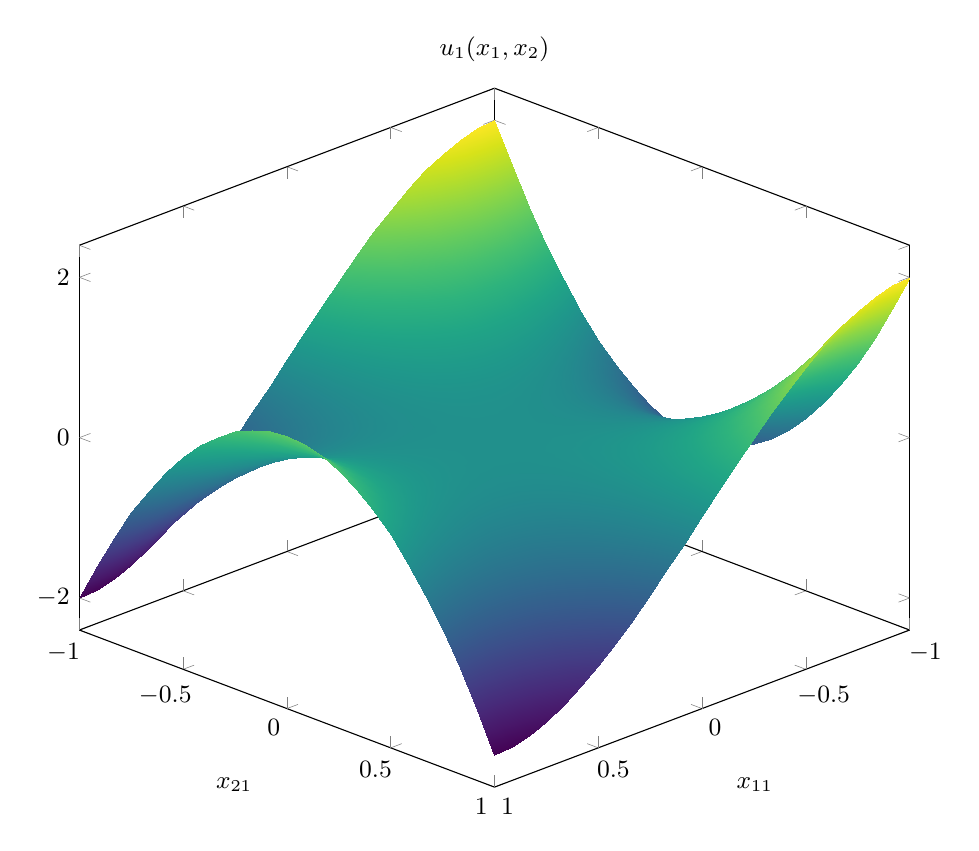
\begin{tikzpicture}
\begin{axis}[
    font=\small,
    domain=-1:1,
    y domain=-1:1,
    xlabel=$x_{11}$,
    ylabel=$x_{21}$,
    title={$u_1(x_1,x_2)$},
    colormap/viridis,
    view={135}{30},
    mesh/ordering=y varies,
    width=\textwidth,
]
\addplot3[
    surf,
    shader=interp,
]
{x^3-3*x*y^2};
\end{axis}
\end{tikzpicture}
\end{minipage}

\begin{example}\label{ex.misc.mul.div}
A general-sum 2-player game in $1 \times 1$ variables on the interval
$$x_{i1} \in [-3,-1] \quad \forall i \in \{1,2\}.$$
The utility functions are given by
\begin{align*}
u_{1}\left( x_{1}, x_{2} \right) &=  - 2 x_{11} x_{21} \\
u_{2}\left( x_{1}, x_{2} \right) &= \frac{2 x_{11}}{x_{21}}.
\end{align*}
The game has a pure Nash equilibrium $x^\star = (-1, -1)$.
\end{example}
\fi

\begin{example}\label{ex.nguyen23.iv}
A 6-player game in $1 \times 1 \times 1 \times 1 \times 1 \times 1$ variables
on the interval
$$x_{i1} \in [x_{\min},x_{\max}] \quad \forall i \in \{1,\dots,6\}.$$
The utility functions are defined by:
$$
u_i(x) = -\eta_ix_{i1}+\beta_i \left(\ln \left(1+a_i\frac{\gamma_i(x)}{1-\Phi_{ii}\gamma_i(x)} \right)-x_{i1}\right) \quad \forall i \in \{1,\dots,6\},
$$
where $\eta_i$, $\beta_i$, and $a_i$ are channel-specific parameters. The parameter $\gamma_i(x)$ represents the \textsc{osnr} \cite{osnr}, defined as
$$
\gamma_i(x) = \frac{x_{i1}}{n_0+\sum_j\Phi_{ij}x_{j1}},
$$
for a given system matrix $\Phi$ and input noise $n_0$. The numerical setting is adopted from an article by \textcite{nguyen.bianchi.ea:nash}. Specifically, $n_0=0.43\times10^{-6}$, $\eta_1=\dots=\eta_6=1$,
\begin{align*}
    \beta & = [0.5, 0.51, 0.52, 0.3, 0.31, 0.32],\\ a & = [0.261, 0.494, 0.107, 0.366, 0.208, 0.305],
\end{align*}
 $x_{\min} = 0.2$, $x_{\max} = 2$, and the matrix
\[
\Phi = \begin{bmatrix}
7.463 & 7.378 & 7.293 & 7.210 & 7.127 & 6.965 \\
7.451 & 7.365 & 7.281 & 7.198 & 7.115 & 6.953 \\
7.438 & 7.353 & 7.269 & 7.186 & 7.103 & 6.942 \\
7.427 & 7.342 & 7.258 & 7.175 & 7.093 & 6.931 \\
7.409 & 7.324 & 7.240 & 7.157 & 7.075 & 6.914 \\
7.387 & 7.303 & 7.219 & 7.136 & 7.055 & 6.894
\end{bmatrix}
\times 10^{-5}.
\]
The game has a Nash equilibrium $x^\star \approx [0.3329, 0.3375, 0.3412, 0.2305, 0.2361, 0.2421]$.
\end{example}
